\chapter{Material models and parameters}
\label{model-parameters}

The engineered tendon construct is $12$ mm in length and
$1\;\mathrm{mm}^2$ in area. In this paper an internal energy
density for the solid phase based upon the worm-like chain model
is used. The reader is directed to \citet{Riefetal:97} and
\cite{Bustamanteetal:2003} where the one-dimensional version of
this model has been applied to long chain molecules. It has been
described and implemented into an anisotropic representative
volume element by \citet{Bischoffetal:2002}, and is summarized
here. The internal energy density of a single constituent chain of
an eight-chain model (Figure \ref{eightchain}) is,
\begin{eqnarray}
\bar{\rho}_0^\mathrm{s}\hat{e}^\mathrm{s}(\bF^{\mathrm{e}^\mathrm{s}},\rho_0^\mathrm{s},\eta^\mathrm{s})
&=& \frac{N k \theta}{4 A}\left(\frac{r^2}{2L} +
\frac{L}{4(1-r/L)} -
\frac{r}{4}\right)\nonumber\\
&-&\frac{N k \theta}{4\sqrt{2L/A}}\left(\sqrt{\frac{2A}{L}} +
\frac{1}{4(1 - \sqrt{2A/L})} -\frac{1}{4} \right)\log(\lambda_1^{a^2}\lambda_2^{b^2}\lambda_3^{c^2})\nonumber\\
&+& \frac{\gamma}{\beta}({J^{\mathrm{e}^\mathrm{s}}}^{-2\beta} -1)
+ 2\gamma{\bf 1}\colon\bE^{\mathrm{e}^\mathrm{s}} \label{wlcmeq}
\end{eqnarray}
\noindent Here, $N$ is the density of chains, $k$ is the Boltzmann
constant, $r$ is the end-to-end length of a chain, $L$ is the
fully-extended length, and $A$ is the persistence length that
measures the degree to which the chain departs from a straight
line. The preferred orientation of tendon collagen is described by
an anisotropic unit cell with sides $a,b$ and $c$---see Figure
\ref{eightchain}. All lengths in this model have been rendered
non-dimensional (Table \ref{mattab}) by dividing by the link
length in a chain.
\begin{figure}[ht]
\psfrag{A}{$a$} \psfrag{B}{$b$} \psfrag{C}{$c$} \centering
{\includegraphics[width=3.5cm]{images/elucidation/wlcm-cuboid.eps}} \caption{Worm-like
chains grouped into an initially anisotropic eight-chain model.}
\label{eightchain}.
\end{figure}

The elastic stretches along the unit cell axes are respectively
denoted $\lambda^\mathrm{e}_1,\lambda^\mathrm{e}_2$ and
$\lambda^\mathrm{e}_3$, and $\bE^{\mathrm{e}^\mathrm{s}} =
\frac{1}{2}(\bC^{\mathrm{e}^\mathrm{s}} - {\bf 1})$ is the elastic
Lagrange strain. The factors $\gamma$ and $\beta$ control bulk
compressibility. The end-to-end length is given by

\begin{equation}
r =
\frac{1}{2}\sqrt{a^2\lambda_1^{\mathrm{e}^2}+b^2\lambda_2^{\mathrm{e}^2}+c^2\lambda_3^{\mathrm{e}^2}},\quad
\lambda_I^{\mathrm{e}} = \sqrt{\bN_I\cdot\bC^{\mathrm{e}}\bN_I}
\label{rwlcm}
\end{equation}

Preliminary mechanical tests of the engineered tendon have been
carried out in our laboratory but, at this stage, the worm-like
chain model has not been calibrated to these tests. Instead,
published data for the worm-like chain, obtained by calibrating
against rat cardiac tissue  \citep{Bischoffetal:2002}, has been
employed.

The fluid phase was modelled as an ideal, nearly-incompressible
fluid:
\begin{equation}
\bar{\rho}^\mathrm{f}_0\hat{e}^\mathrm{f}(\bF^{\mathrm{e}^\mathrm{f}},\rho_0^\mathrm{f},\eta^\mathrm{f})
=
\frac{1}{2}\kappa(\mathrm{det}(\bF^{\mathrm{e}^\mathrm{f}})-1)^2,
\end{equation}

\noindent where $\kappa$ is the fluid bulk modulus.

Only a solid and a fluid phase were included for the tissue. Low
values were chosen for the mobilities of the fluid
\citep{Swartzetal:99} with respect to the solid phase (see Table
\ref{mattab}). In order to demonstrate growth, the solid phase
must have a source term, $\Pi^\mathrm{s}$ (Section \ref{sect2}),
and the only other phase, the fluid, must have $\Pi^\mathrm{f} =
-\Pi^\mathrm{s}$. Therefore, contrary to the case made in Section
\ref{sect2}, a non-zero value of the fluid source,
$\Pi^\mathrm{f}$, was assumed. A form motivated by first-order
reactions was used:
\begin{equation}
\Pi^\mathrm{f} = -k^\mathrm{f}(\rho_0^\mathrm{f} -
\rho_{0_\mathrm{ini}}^\mathrm{f}),\quad \Pi^\mathrm{s} =
-\Pi^\mathrm{f}, \label{piform}
\end{equation}

\noindent where $k^\mathrm{f}$ is the reaction rate, and
$\rho_{0_\mathrm{ini}}^\mathrm{f}$ is the initial fluid
concentration. This term acts as a source for the solid when
$\rho_0^\mathrm{f}
> \rho_{0_\mathrm{ini}}^\mathrm{f}$, and a sink when
$\rho_0^\mathrm{f} < \rho_{0_\mathrm{ini}}^\mathrm{f}$.

In a very simple approximation, the fluid's mixing entropy was
written as
\begin{equation}
\eta^\mathrm{f}_\mathrm{mix} =
-\frac{k}{\sM^\mathrm{f}}\log\frac{\rho_0^\mathrm{f}}{\rho_0}.
\label{mixentropy}
\end{equation}

\noindent Recall that in the notation of Section \ref{sect2},
$\sM^\mathrm{f}$ is the fluid's molecular weight.

\begin{table}[ht]
\caption{Material parameters used in the analysis} \label{mattab}
\begin{tabular}{lcll}
\hline
\multicolumn{1}{c}{Parameter} & Symbol & Value & Units\\
\hline
Chain density & $N$ & $7\times 10^{21}$ & $\mathrm{m}^{-3}$\\
Temperature& $\theta$  & $310.0$ & K\\
Persistence length & $A$ & $1.3775$ & --\\
Fully-stretched length & $L$ & $25.277$ & --\\
Unit cell axes & $a,\;b,\;,c$ & $9.2981,\;12.398,\;6.1968$ & --\\
Bulk compressibility factors & $\gamma,\;\beta$ & $1000,\; 4.5$ & --\\
Fluid bulk modulus &$\kappa$ & $1$ & GPa\\
Fluid mobility tensor components& $D_{11},\;D_{22},\;D_{33}$ & $1\times 10^{-8},\;1\times 10^{-8},\;1\times 10^{-8}$ &$\mathrm{m}^{-2}\mathrm{sec}$\\
Fluid conversion reaction rate & $k^\mathrm{f}$ & $-1.\times 10^{-7}$ & $\mathrm{sec}^{-1}$\\
Gravitational acceleration & $\bg$ & $9.81$ & $\mathrm{m}.\mathrm{sec}^{-2}$\\
Molecular weight of fluid &$\sM^\mathrm{f}$& $2.9885\times 10^{-23}$ & $\mathrm{kg}$\\
\hline
\end{tabular}
\end{table}
